\section{Inicialización}

La inicialización del conjunto de soluciones inicial es determinado de manera aleatoria. De tal forma de tener contar con distintos lugares del espacio de búsqueda. Cada solución del conjunto contiene un conjunto de rutas, escogido de la siguiente manera: aleatoriamente se escoge un largo de ruta, el cual está comprendido entre el mínimo y máximo establecido. Se escoge aleatoriemente un punto de partida y se genera un camino mediante las conexiones con paradas vecinas hasta completar el largo. Se realiza este procedimiento hasta tener un conjunto de rutas que posea todos los paraderos disponibles o hasta que se agote un número de intentos, lo que puede ocurrir cuando el número de paraderos es muy grande en comparación con la cantidad de paraderos que serán destinados a una ruta o si el número de rutas a generar es muy pequeño. Las instancias con las que se trabajará siempre tratarán de incluír a todos los paraderos.\\

Se genera una población de soluciones de manera de tener varias soluciones candidatas. Este conjunto de soluciones inciales es un conjunto de soluciones factible, lo que quiere decir que las rutas generadas son conexas y además no presentan ciclos ni backtrackings. El algoritmo trabaja con soluciones factibles y al generar nuevas soluciones se comprueban las condiciones necesarias para que también sean factibles. 

\section{Proceso de transformación}

\subsection{Selección de soluciones}

El primer paso en el proceso de transformación del algoritmo consiste en realizar una selección clonal. Esto es, seleccionar a los mejores anticuerpos en base a una función de aptitud (\ref{eq:faptitud}). 

\begin{equation}
\label{eq:faptitud}
f_{aptitud}=\alpha \cdot FO_1 + \beta \cdot FO_2
\end{equation}

Donde $FO_1$ y $FO_2$ corresponden a las funciones objetivo dadas por las ecuaciones (\ref{eq:fo1}) y (\ref{eq:fo2}), respectivamente. Un porcentaje de estas soluciones son escogidas de acuerdo al resultado de $f_{aptitud}$ para pasar a la siguiente etapa del algoritmo.

\subsection{Operadores de transformación}

Los mejores anticuerpos son clonados hasta llegar a una cierta población. Esto consiste básicamente en generar muchas copias de los mejores anticuerpos. El operador de selección toma un anticuerpo y genera uno igual. La manera de decidir cual de los mejores anticuerpos se clona se realiza de manera aleatoria. De esta forma cada uno de los anticuerpos tiene la misma probabilidad de ser clonado.\\

Posteriormente, se utiliza un operador de mutación, el cual consiste en introducir pequeños cambios al conjunto de rutas para producir cambios en sus funciones objetivo, y por ende en la función de aptitud. La mutación consiste en seleccionar aleatoriamente una ruta de una solucion e introducir un nuevo vertice en ella, siempre y cuando no exceda el límite superior.


\subsection{Selección de soluciones para conformar nueva población}

Luego, se aplica una reducción de la población de los clones, dejando los más aptos (con una mejor función de aptitud). Se procede a reemplazar a los peores anticuerpos con anticuerpos generados aleatoriamente, siguiendo las mismas restricciones de la generación inicial al generar soluciones candidatas factibles. 



\section{Sintonización de Parámetros}

Para la sintonización de parámetros se escogieron 4 de los parámetros y el resto quedó con un valor fijo. Entre los parámetros con valor fijo se utilizaron los valores de la Tabla \ref{tab:paramfijos}. La instancia utilizada fue la de \texttt{Mandl 6:2:8}, cuyo grafo está representado en la Figura \ref{fig:mandl}. Se buscan 6 rutas con longitudes que varían en el rango de 2 a 8 paradas.

\begin{table}[!htb]
\begin{center}
\begin{tabular}{|c|c|}
\hline
\texttt{ALPHA} & 1.0\\ \hline
\texttt{BETA} & 1.0\\ \hline
\texttt{AFINIDAD} & 1\\ \hline
\texttt{REEMPLAZO} & 0.01\\ \hline
\end{tabular}
\label{tab:paramfijos}
\caption{Parámetros seteados en un valor fijo para Mandl.}
\end{center}
\end{table}

Los parámetros \texttt{POP\_SIZE}, \texttt{CLON\_SIZE}, \texttt{GENERACIONES} y \texttt{CLONES} fueron puestos a prueba al utilizar ParamILS, un sintonizador de parámetros que utiliza un intérprete del código y ejecuta el algoritmo utilizando un rango de valores para los 4 parámetros escogidos.

\begin{figure}[!htb]
\begin{verbatim}
ps {20, 40, 100, 160, 200}[100]
cs {5, 15, 25}[15]
it {10, 30, 50, 70, 100}[30]
pc {10, 30, 50}[10]
\end{verbatim}
\caption{Valores utilizados en los parámetros sintonizados en Mandl.}
\label{fig:paramsintonizados}
\end{figure}

En la Figura \ref{fig:paramsintonizados} \texttt{ps}, \texttt{cs}, \texttt{it} y \texttt{pc} corresponden a \texttt{POP\_SIZE}, \texttt{CLON\_SIZE}, \texttt{GENERACIONES} y \texttt{CLONES} respectivamente.

\newpage

Al ejecutar ParamILS se obtuvo la siguiente salida:

\begin{small}
\begin{verbatim}
Final best parameter configuration: cs=5, it=100, pc=10, ps=200
==================================================================
Active parameters: cs=5, it=100, pc=10, ps=200
==================================================================
Training quality of this final best found parameter configuration: 
-704.619631901841, based on 163 runs with cutoff 1000000000.0
Test quality of this final best found parameter configuration: 
-703.96, based on 50 independent runs with cutoff 1000000000.0
\end{verbatim}
\end{small}

Para este valores de parámetros se obtuvo un valor máximo de hipervolumen igual a 703.96.

\section{Experimentos}

El experimento con los valores de parámetros fijados según la Tabla \ref{tab:paramfijos} y los obtenidos mediante ParamILS, según lo mostroado a continuación:

\begin{table}[!htb]
\begin{center}
\begin{tabular}{|c|c|}
\hline
POP SIZE & 200\\ \hline
ALPHA & 1.0\\ \hline
BETA & 1.0\\ \hline
CLON SIZE & 5\\ \hline
AFINIDAD & 1\\ \hline
GENERACIONES & 100\\ \hline
CLONES & 0.1\\ \hline
REEMPLAZO & 0.01\\ \hline
\end{tabular}
\caption{Valores utilizados para el experimento con la instancia de Mandl.}
\end{center}
\end{table}

Notar que el porcentaje de clones fue manejado en ParamILS con valores entre 0 y 100 y pasado posteriormente a valores entre 0 y 1.

\begin{figure}[!htb]
\begin{center}
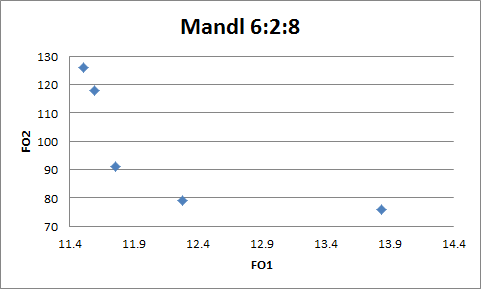
\includegraphics[scale=0.7]{pareto_mandl.png}
\caption{Frente de Pareto de la instancia de Mandl.}
\label{fig:pareto_mandl}
\end{center}
\end{figure}

\begin{table}[!htb]
\begin{center}
\begin{tabular}{|l|c|}
\hline
Hipervolumen & 698.452\\ \hline
Tiempo de ejecución & 23 segundos\\ \hline
\end{tabular}
\caption{Hipervolumen y tiempo de ejecución.}
\label{tab:mandldata}
\end{center}
\end{table}

Además, los mejores valores para las funciones objetivo corresponden a:
\begin{itemize}
\item Mejor FO1: 11.5087
\item Mejor FO2: 76
\end{itemize}

\newpage
El conjunto de rutas que presenta el menor valor para la función de aptitud se muestra a continuación:
\begin{verbatim}
6-3
9-15-6-8
3-2-4-12
8-6-3
8-15-7-10-14-13-11
1-2-5
\end{verbatim}

Se puede concluir que estos resultados no reflejan exactamente a lo obtenido mediante la sintonización de parámetros porque esto corresponde solo a una ejecución del algoritmo. Por otra parte, ParamILS realiza una cantidad considerable de experimentos probando con distintos valores y logra encontrar el mejor valor de hipervolumen. En este caso el valor es cercano al mejor valor obtenido, sin embargo si se realizara otro experimento podría originar un valor más cercano o más lejano.

\section{Conclusiones}

Los algoritmos inmunes artificiales utilizan analogías de los organismos vivos. Cuando un virus ataca al organismo los anticuerpos son capaces de interactuar con este y los más capaces son duplicados para atacar y eliminar a una enfermedad que cause. Luego se guarda en memoria una cantidad menor de este anticuerpo para que esté preparado a nuevas infecciones del mismo virus o uno similar. Esta idea es la que permite encontrar soluciones mediante la clonación y mutación de los mejores individuos. El proceso de búsqueda de soluciones es un proceso adaptativo, lo que quiere decir que los anticuerpos se capacitan para enfrentarse a infecciones futuras. \\

Mediante esta implementación, la cual está compuesta por variables, restricciones, funciones objetivo, función de aptitud, operadores de selección y transformación para una población de anticuerpos se pudo encontrar un conjunto de soluciones no dominadas según Pareto, obteniendo mejores soluciones en tiempos relativamente cortos. \\

El proceso de sintonización de parámetros fue útil para poder encontrar valores para parámetros y obtener un mejor resultado, el cual está reflejado en un mayor valor de hipervolumen.\\
